\documentclass[10pt, notitlepage]{article}
\usepackage[utf8]{inputenc}
\usepackage[english]{babel}
\usepackage[letterpaper, margin=0.2in]{geometry}
\usepackage{amsmath, amssymb, amsfonts}
\usepackage{enumitem}
\usepackage{hyperref}
\usepackage{csquotes}
\usepackage{graphicx}
\usepackage{caption}
\usepackage{subcaption}
\usepackage{titlesec}
\usepackage{titling}
\usepackage{fancyhdr}
\usepackage{enumitem}
\usepackage[backend=biber, style=numeric, sorting=ynt]{biblatex}
\addbibresource{writeups/proposalCitations.bib}
\nocite{*}

\newcommand{\dt}{\textbullet}

\setlength{\droptitle}{-50pt}

\pagestyle{empty}

%opening
\title{\textbf{Sokoban Solver}}
\author{Benjamin Huang, Yen-shi Wang, and Zachary Armendariz}
\date{}

\begin{document}

\maketitle

\vspace*{-55pt}

\section*{Project Proposal}
\begin{itemize}
    \item \textbf{What is the application domain/area?} In the domain of Artificial Intelligence, search and game theory are always popular research topics. For this project, we aim to design better kernels according to hardware architecture to solve Sokoban, which is a well-known puzzle since 1982.
    
    \item \textbf{What is the proposed computation problem?} Sokoban is a puzzle game, involving a character packing boxes in a warehouse. The objective is to move boxes from their starting locations onto the designated positions in the warehouse. The character can only push boxes from adjacent squares in the direction of the box from the character. Often, the warehouse layout is oddly shaped, providing a challenge since pushing a box the wrong way will often result in it being stuck in a corner, and pushing a box the right way requires the character to be positioned correctly.
    
    Finding a solution is PSPACE-complete. Currently, the best available solver (Takaken) is only able to solve 86 of 90 levels in the standard test suite, known as XSokoban.
    
    Solving a Sokoban puzzle is essentially a graph search problem. From the initial state, a program branches out to all possible future states. Because of the sheer complexity of the problem, a fair number of pruning techniques are needed to ensure that solvers are not simply doing a brute-force search. This provides many areas for optimization.
    
    A faster solver would be able to explore more of the search tree, which would enable it to find solutions more quickly. Typically, puzzle solve time is on the order of seconds to hundreds of seconds, depending on the difficulty.

    
    \item \textbf{What is the state-of-the-art? Is there a standard or algorithm?}
    \begin{itemize}
        \item \href{https://webdocs.cs.ualberta.ca/~games/Sokoban/program.html}{Rolling Stone}. This is a 2004 solver. It is open source and written in C. It solves 57 of 90 puzzles in the standard test suite.
        \item \href{http://sokobano.de/wiki/index.php?title=JSoko_Solver}{JSoko}. This is a current game and solver package written in Java. It is an open source project. It can solve 67 of the 90 puzzles in the standard test suite.
        \item \href{http://sourceforge.net/projects/sokobanyasc/}{YASS}. This is a current game and solver package written in Delphi/Kylix. It is an open source project. It can solve 84 of the 90 puzzles in the standard test suite.
        \item \href{http://codeanalysis.fr/sokoban/}{Sokolution}. This is a current solver. It is not open-source and runs on Windows. It can solve 80 out of the 90 standard puzzles.
    \end{itemize}
    
    The common techniques used to solve Sokoban can be categorized into data structures, search algorithms, and pruning methods.
    
    \begin{itemize}
        \item Data structures: hash table for each state, transposition tables, normalized player position.
        \item Search algorithms: BFS, DFS, iterative deepening, a-star search, and Bi-directional BFS.
        \item Pruning methos: dead lock, PI-Corrals.
    \end{itemize}

    \item \textbf{What is the scale? How much data? About the deadline?} There are about 4000 puzzles that can be used for benchmarking. Most of them can be downloaded from Sokoban Wiki.

    \item \textbf{What is the end product you are expecting to deliver?} The first phrase of this project will focus on choosing a baseline solver, determining which algorithm and data structure to be optimized, and collecting benchmarks we need during the entire project.
        
        At the end of the project, we expect both algorithm and data structure run faster on ECE workstation and the amount of improvement can be clearly visualized by charts and statistics. Moreover, there should be a version of solver can support parallel computation.

    \item \textbf{What architecture?} ECE Workstation ece030.ece.local.cmu.edu. 2x Intel Xeon E5 2680, 2x8 cores, 2.7GHz (3.5GHz Turbo), 256GB RAM
    
\end{itemize}

\begin{table}[!htb]
    \begin{minipage}{.6\linewidth}
      \centering
        \begin{tabular}{|l|l|}
            \hline
            \multicolumn{2}{|c|}{Tentative division of labor} \\
            \hline\hline
            Yen-shi Wang              &Deepening A* Search, Deadlock Tables, Goal Cuts\\
            Benjamin Huang            & Minmatching, Tunnel Macros, Goal Macros\\
            Zachary Armendariz \quad  & Hash Tables, Move Ordering, Pattern Searches \\
            \hline
        \end{tabular}
    \end{minipage}%
    \begin{minipage}{.4\linewidth}
        \centering
        \begin{tabular}{|l|l|}
            \hline
            \multicolumn{2}{|c|}{Tentative Meeting Times} \\
            \hline\hline
            1st Preference &Tuesday, 3:00-4:00pm \\
            2nd Preference &Thursday, 5:30-6:30pm \\
            3rd Preference &Friday, 1:00-2:00pm \\
            \hline
        \end{tabular}
    \end{minipage} 
\end{table}
    
\begin{figure}[ht]
\centering
\begin{subfigure}{.22\textwidth}
  \centering
  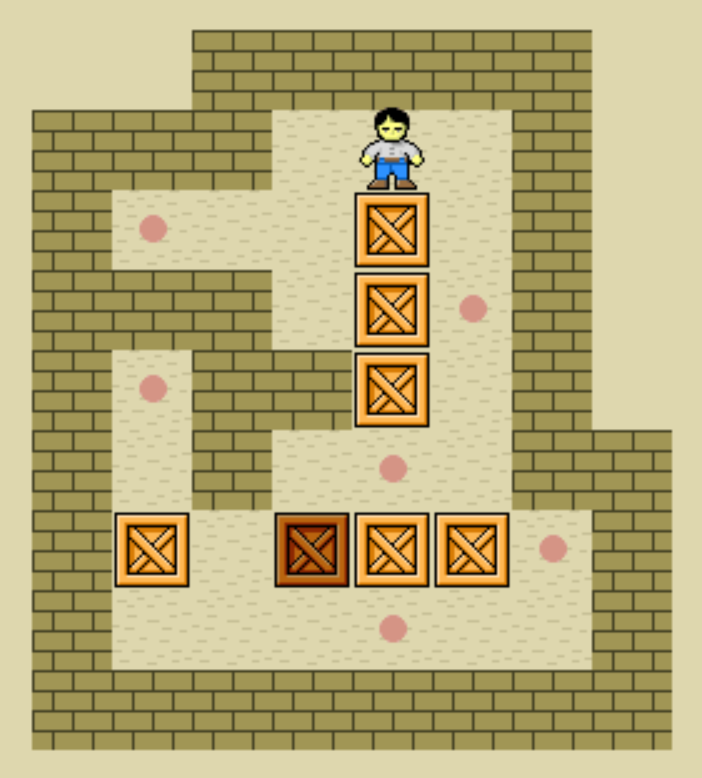
\includegraphics[width=.8\linewidth]{images/sokoban1.png}
  \caption{Start of game}
  \label{fig:sub1}
\end{subfigure}%
\begin{subfigure}{.22\textwidth}
  \centering
  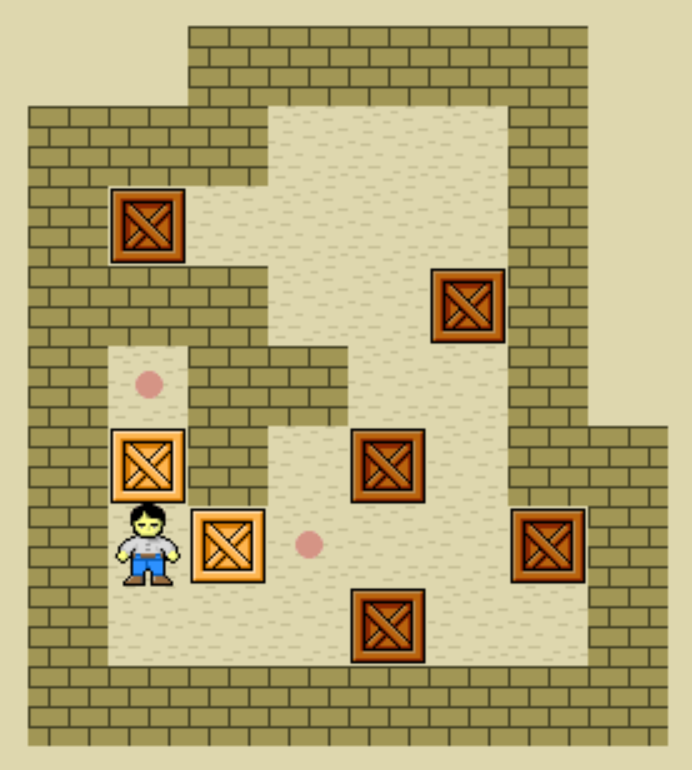
\includegraphics[width=.8\linewidth]{images/sokoban2.png}
  \caption{Near the end of game}
  \label{fig:sub2}
\end{subfigure}
\caption{Screenshots of Sokoban}
\label{fig:test}
\end{figure}

\printbibliography

\end{document}
